\section{Schadensbilder}
\label{sec:schadensbilder}
% Entwurf 2026-10-21 nach der Sichtprüfung des Nutzers (failed_teeth_user.yaml) und den drei von ihm
% genannten Fotos; Nachher-Scans (M5) am 2026-10-21 ausgewertet (scripts/contour_wear.py).

Nach dem Lauf wurden die gelaufenen Räder unter dem Mikroskop aufgenommen und alle Zähne in einer Sichtprüfung bewertet. \figref{fig:schaden_16nm} zeigt je eine Aufnahme der Stufen $8$, $12$ und $16$\,Nm im Stirnschnitt der Verzahnung, \figref{fig:schaden_oberflaeche} eine Flanke der Stufe $16$\,Nm mit der stark aufgerauten Oberfläche. Drei Befunde kehren an allen Rädern wieder. Erstens trägt die belastete Flanke jedes Zahns am unteren Ende des aktiven Profils, $0{,}7$ bis $0{,}8$\,mm über dem Fußkreis, eine Stufe. Die Kopfkante des Ritzels hat sich dort in die Flanke eingearbeitet. Das FE-Modell legt den Kontakt der Ritzelkopfkante bei den isotropen Stufen auf den Radius $25{,}8$\,mm, also $1{,}0$\,mm über den erzeugten Fußkreis von $24{,}76$\,mm, und findet dort die größten Auslastungen des Nachweises (\secref{sec:stommel_global_slife}). Die Konturscans nach dem Lauf legen den Beginn der Stufe rund $0{,}3$\,mm darunter. Zweitens sind die Kopfkanten der Räder bei $16$\,Nm ausgefranst und die Flanken mit freiliegenden Fasern aufgeraut, bei $12$\,Nm schwächer, bei $8$\,Nm kaum. Die Sichtprüfung stuft die Oberfläche der vier Räder der Stufe $16$\,Nm als stark, der Räder bei $12$\,Nm als gering bis mittel und des Rades 97345 bei $8$\,Nm als kaum aufgeraut ein. Drittens brechen die Zähne im Fuß, einzeln wie beim Rad 97345 oder in Gruppen von bis zu acht benachbarten Zähnen (\tabref{tab:versuchsprogramm_pa46}). An drei Rädern der Stufe $16$\,Nm brechen vier Zähne nicht im Fuß, sondern in der Flanke über der Spur der Ritzelkopfkante (97340 Zähne 39 und 40, 97366 Zahn 37, 97355 Zahn 38). Ob der Riss dort in der Stufe beginnt, ist am Mikroskop noch zu klären.

\begin{figure}[htbp]
    \centering
    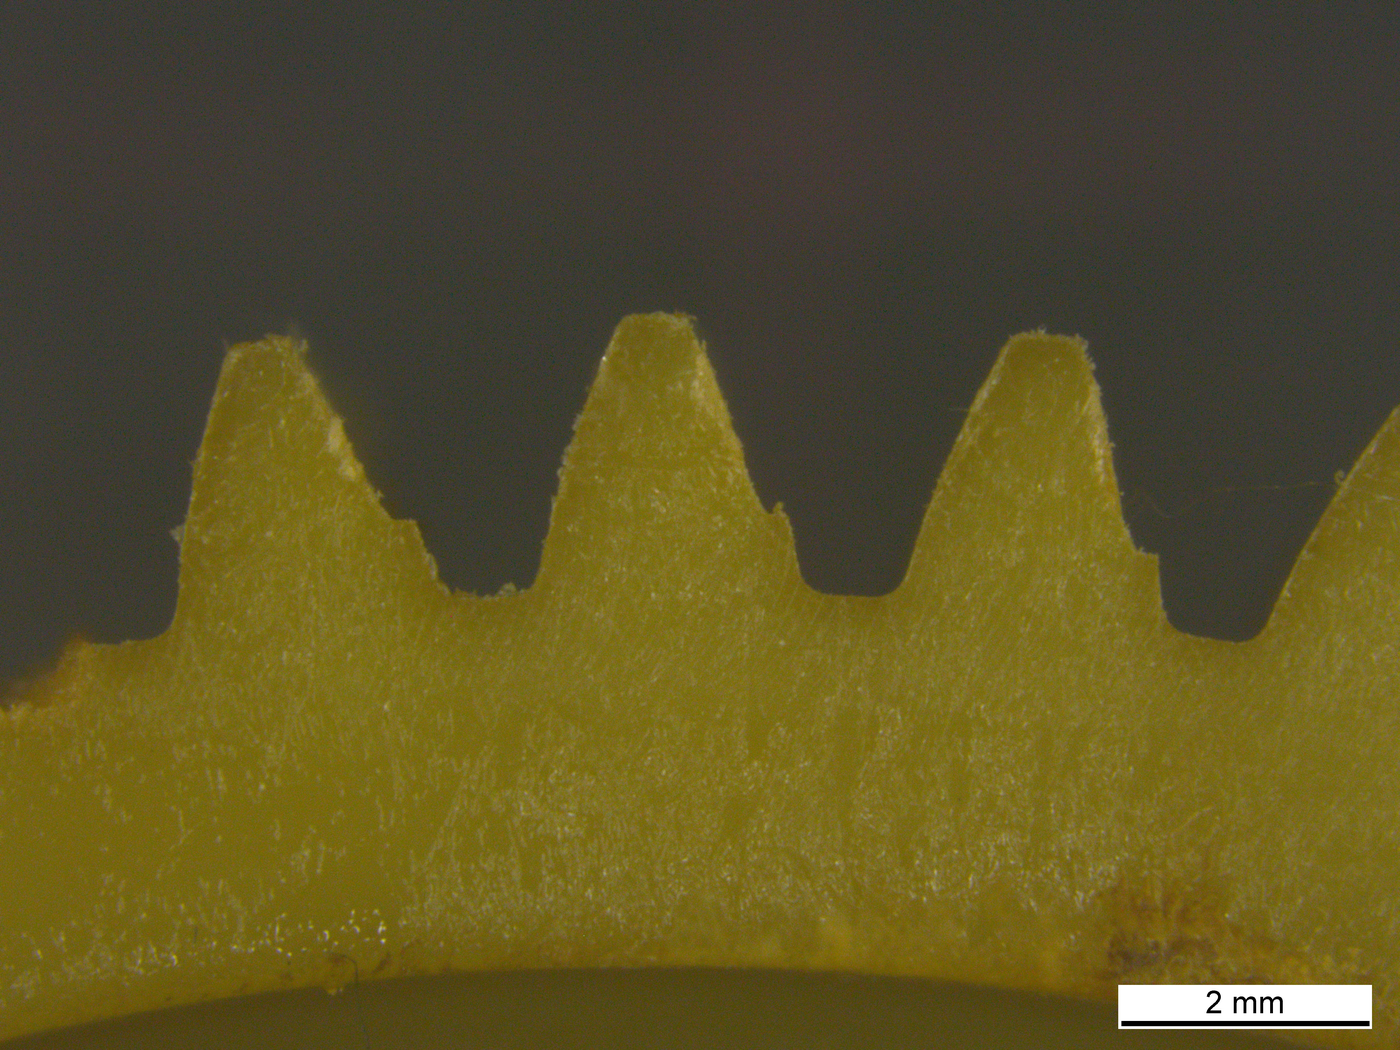
\includegraphics[width=0.48\textwidth]{kap6/schaden_8nm_170824}\hfill
    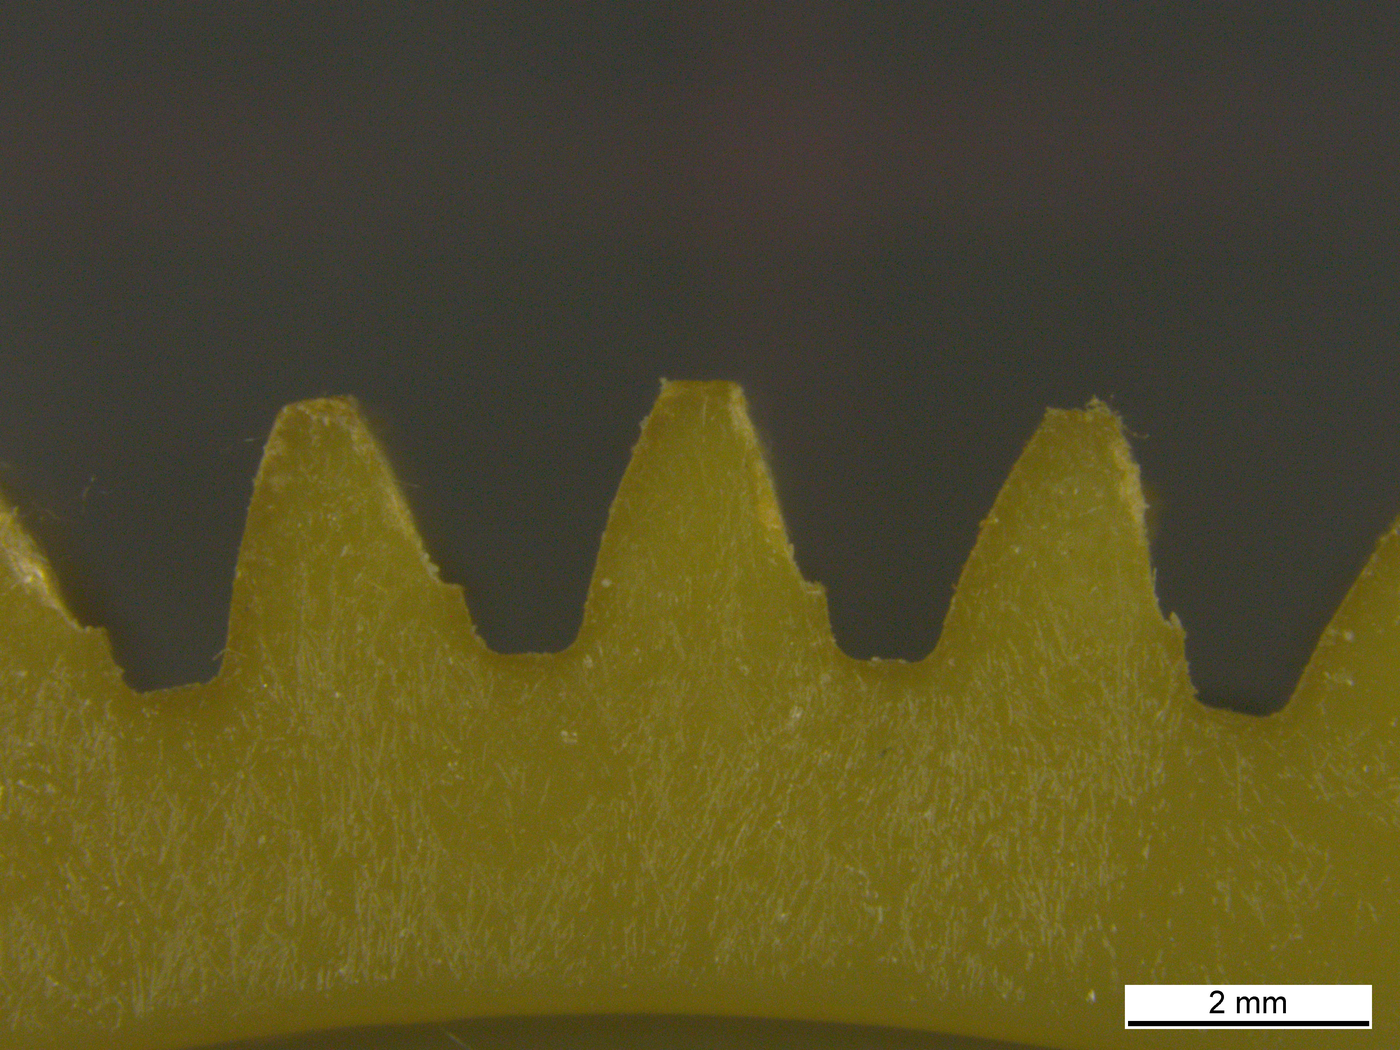
\includegraphics[width=0.48\textwidth]{kap6/schaden_12nm_170817}\\[2pt]
    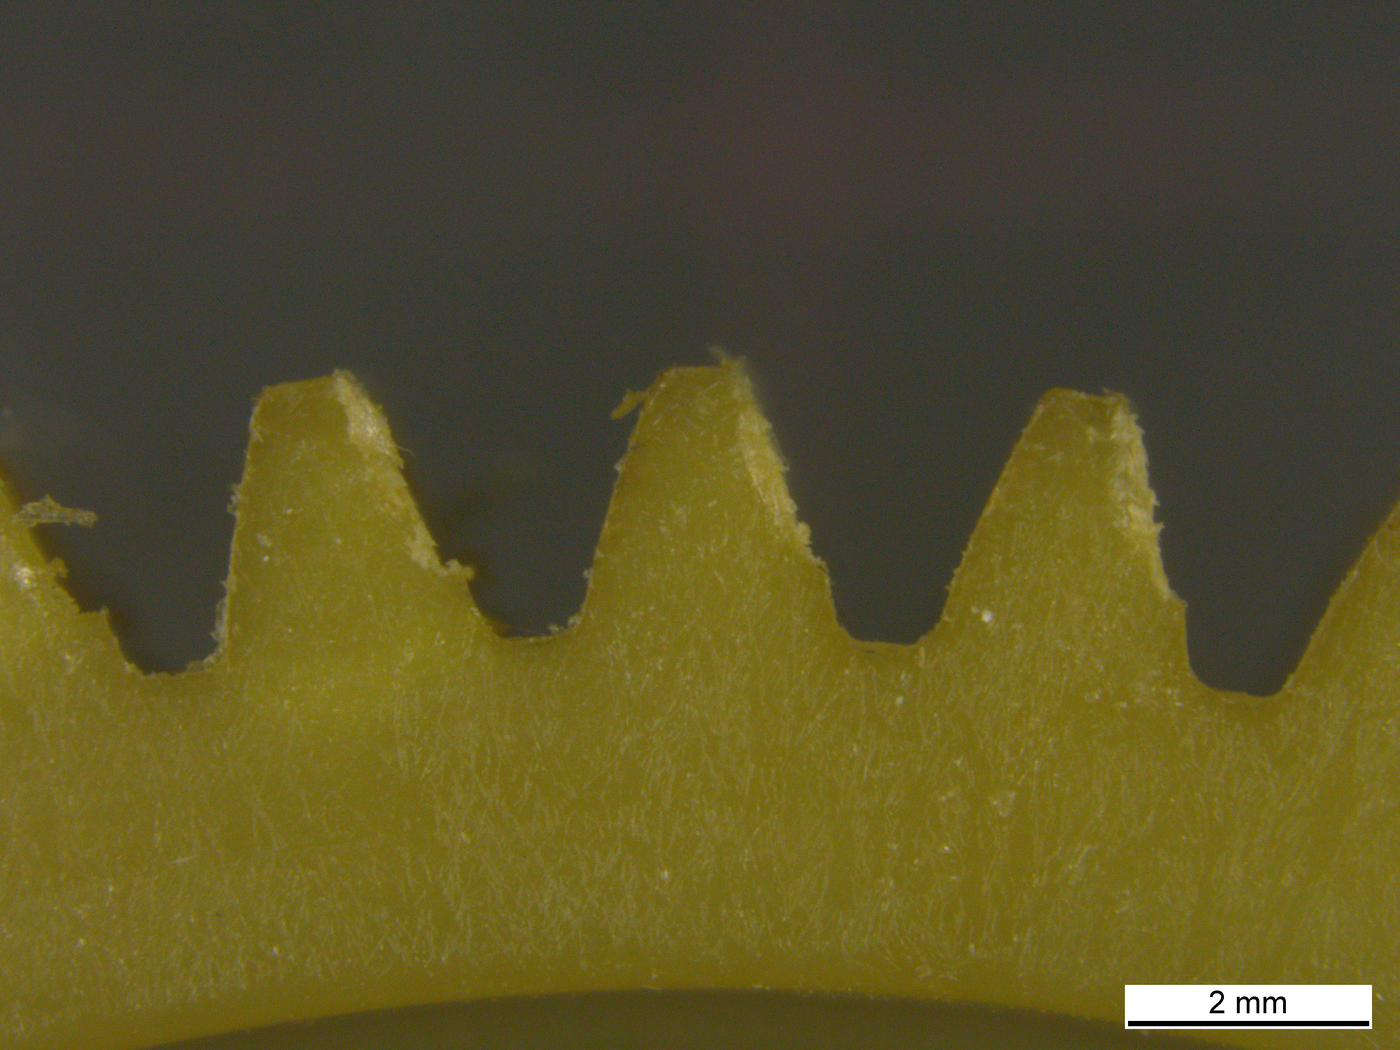
\includegraphics[width=0.48\textwidth]{kap6/schaden_16nm_170820}
    \caption{Gelaufene Räder aus PA46-GF30 im Stirnschnitt unter dem Mikroskop, Maßstab $2$\,mm: Stufe $8$\,Nm (oben links), $12$\,Nm (oben rechts) und $16$\,Nm (unten). An jedem Zahn die Stufe der eingearbeiteten Ritzelkopfkante am unteren Ende des aktiven Profils, bei $16$\,Nm dazu die ausgefransten Kopfkanten.}
    \label{fig:schaden_16nm}
\end{figure}

\begin{figure}[htbp]
    \centering
    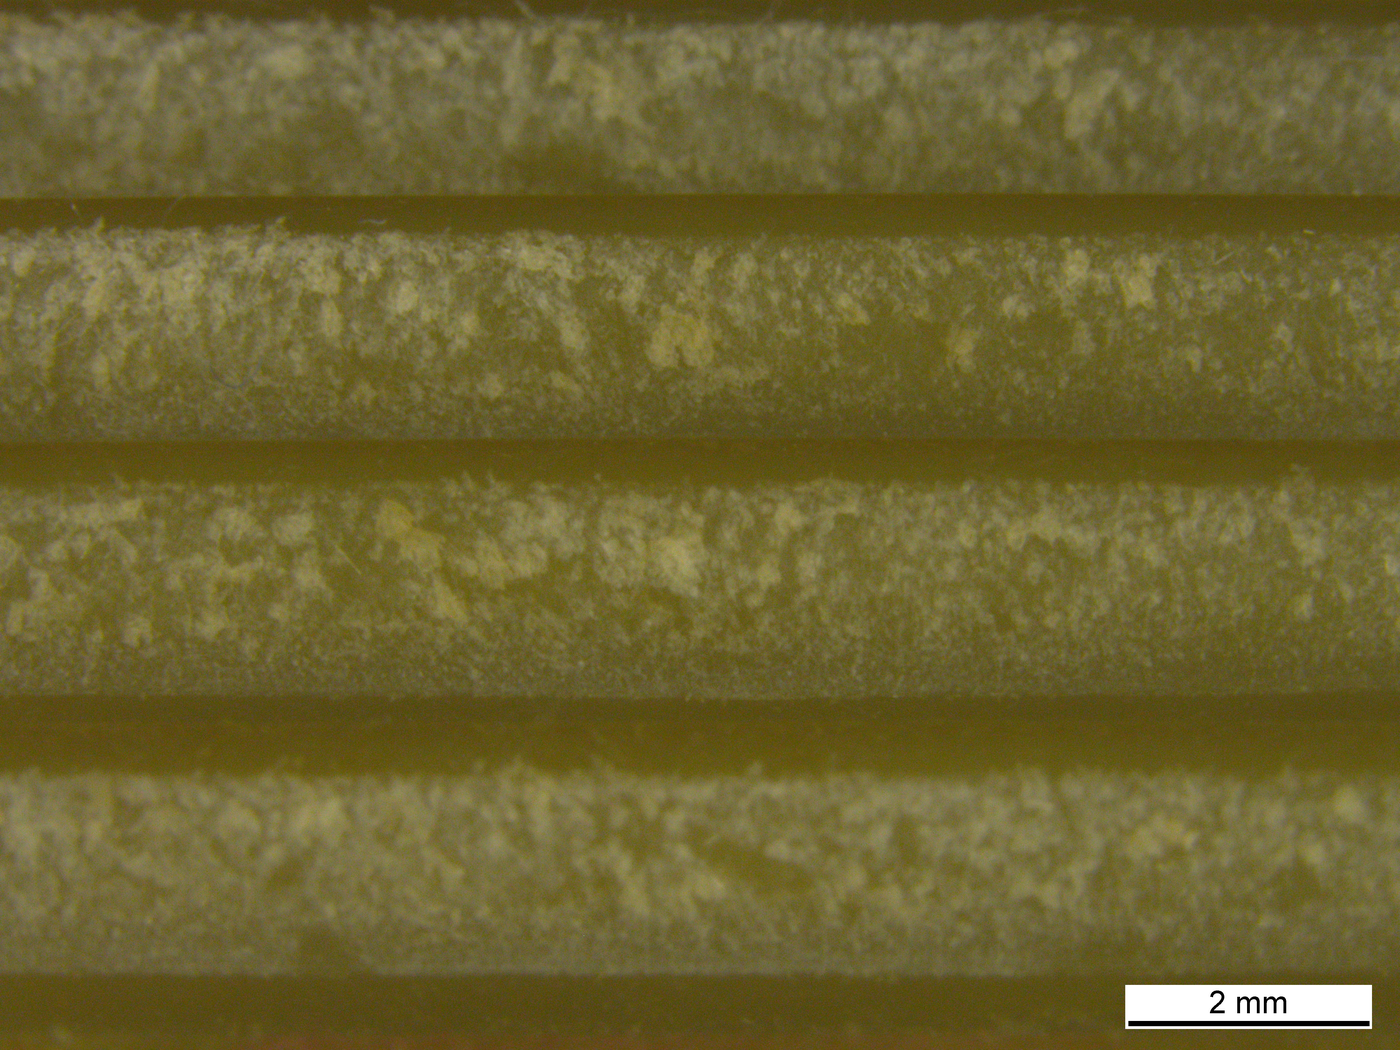
\includegraphics[width=0.62\textwidth]{kap6/schaden_16nm_170810}
    \caption{Aufgeraute Flanke eines Rades der Stufe $16$\,Nm mit freiliegenden Fasern, Maßstab $2$\,mm. Bezug der Einstufung gering, mittel und stark nach der Sichtprüfung in \secref{sec:versuchsprogramm}.}
    \label{fig:schaden_oberflaeche}
\end{figure}

Die Konturscans der Räder 97345 ($8$\,Nm, $24{,}96 \cdot 10^{6}$ Lastwechsel), 97351 ($12$\,Nm, $2{,}42 \cdot 10^{6}$) und 97340 ($16$\,Nm, $1{,}92 \cdot 10^{6}$) nach dem Lauf, gelagert nach \secref{sec:dokumentation_pruefraeder}, machen die Stufe messbar. \figref{fig:verschleiss_profil} trägt die Abweichung der gelaufenen Flanken von der Sollkontur über dem Radius auf, dahinter das Band der 49 Flanken vor dem Lauf, das dieselbe Lagerung mit $6$\,µm RMS in den Fußrundungen trifft. \figref{fig:verschleiss_kontur} zeigt dieselben Zähne auf dem Sollzahn, nicht überhöht. Nur die belastete Flanke ist abgetragen. Die unbelastete Flanke liegt im Mittel innerhalb von $25$\,µm am Band. Der Abtrag beginnt an allen Zähnen zwischen $r = 25{,}42$ und $25{,}45$\,mm mit einer steilen Stufe und bleibt von dort bis zum Kopf nahezu gleichmäßig, im Mittel über das aktive Profil $156$ bis $197$\,µm bei $8$\,Nm, $95$ bis $128$\,µm bei $12$\,Nm und $46$ bis $89$\,µm bei $16$\,Nm (\tabref{tab:verschleiss}). Das Maximum liegt $10$ bis $60$\,µm über dem Mittel zwischen $r = 25{,}7$ und $26{,}4$\,mm. Die Grundzahndicke aus den Evolventen bestätigt die Summe. Sie ist um $16$ bis $235$\,µm kleiner als das Mittel der Räder vor dem Lauf. Auf die Lastwechsel bezogen trägt der Lauf bei $8$\,Nm $6$ bis $8$\,µm je Million ab, bei $12$\,Nm $39$ bis $53$\,µm und bei $16$\,Nm $24$ bis $46$\,µm. Die Kopfrundung der belasteten Seite misst nach dem Lauf $0{,}03$ bis $0{,}12$\,mm statt $0{,}21$\,mm, die der unbelasteten Seite ist unverändert. Der Beginn der Verschleißzone liegt rund $0{,}2$\,mm unter dem rechnerischen Fußnutzkreis von $25{,}66$\,mm und rund $0{,}4$\,mm unter der Knotenreihe des Kantenkontakts im FE-Modell ($25{,}80$\,mm). Der Eingriff beginnt im Lauf also tiefer auf der Flanke, als die Geometrie der unverformten Paarung angibt. Im FE-Modell reicht der Kontakt der gerundeten Ritzelkopfkante über alle 99 Stellungen bis $r = 25{,}60$\,mm hinab, gelesen an den Flankenknoten des Zahns T3 mit einer kleinsten Hauptspannung unter $-15$\,MPa. Zahnverformung und Kantenrundung verlegen den Beginn dort um $0{,}06$\,mm unter den Nutzkreis, der Lauf um weitere $0{,}15$ bis $0{,}18$\,mm. Die im Fuß gebrochenen Zähne 36 und 37 des Rades 97340 zeigen im Scan Bruchflächen und bleiben außer Betracht.

\begin{figure}[htbp]
    \centering
    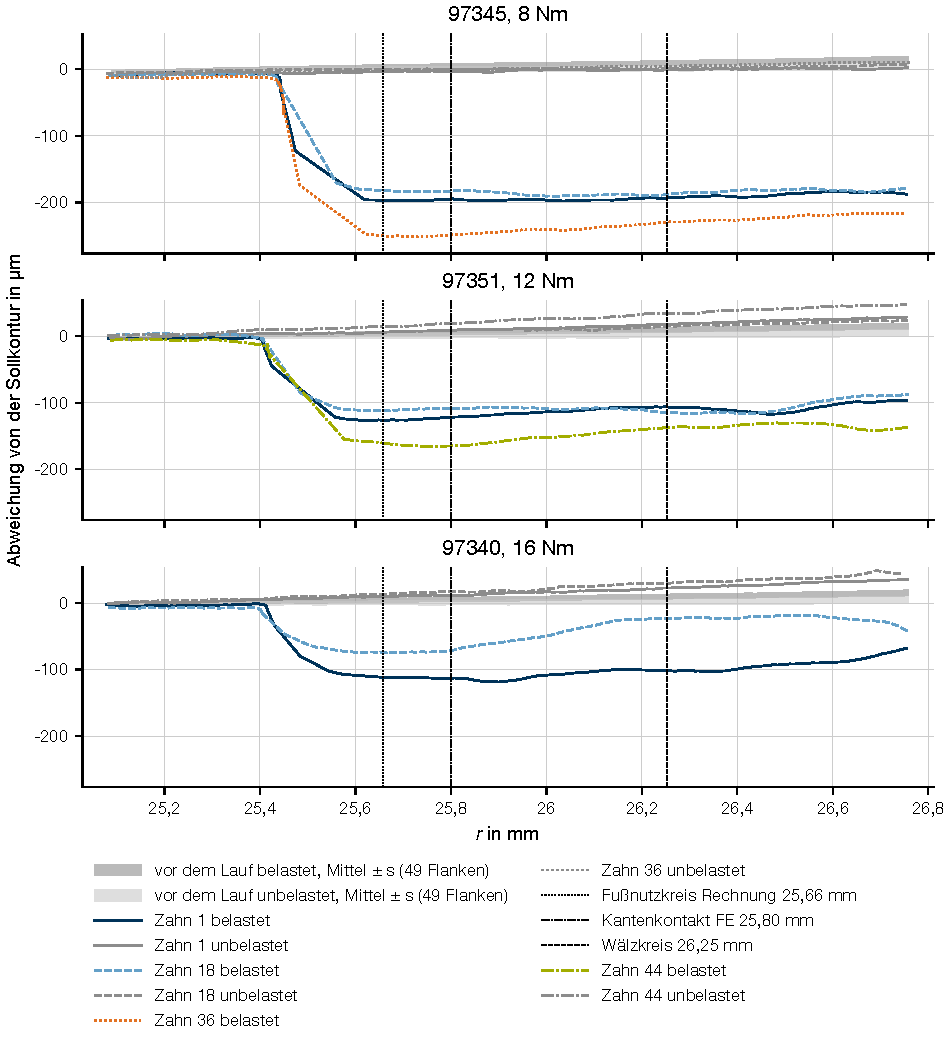
\includegraphics[width=\textwidth]{kap6/verschleiss_profil}
    \caption{Abweichung der gelaufenen Flanken von der Sollkontur über dem Radius für die Räder 97345 ($8$\,Nm), 97351 ($12$\,Nm) und 97340 ($16$\,Nm), je gescannter Zahn ein Strichmuster, die belastete Flanke farbig und die unbelastete grau, dahinter das Band aus Mittel und Standardabweichung der 49 Flanken vor dem Lauf. Senkrecht der rechnerische Fußnutzkreis, die Knotenreihe des Kantenkontakts im FE-Modell und der Wälzkreis.}
    \label{fig:verschleiss_profil}
\end{figure}

\begin{figure}[htbp]
    \centering
    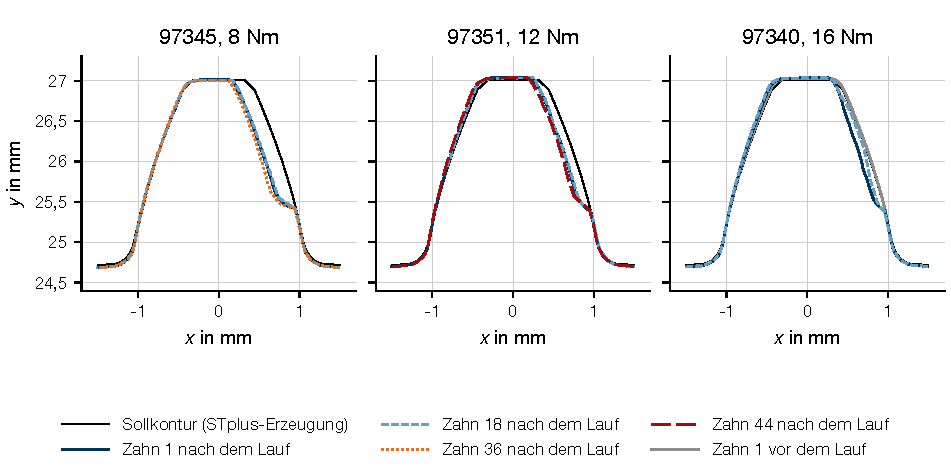
\includegraphics[width=\textwidth]{kap6/verschleiss_kontur}
    \caption{Gelaufene Zähne auf dem Sollzahn der Erzeugung, Abweichung nicht überhöht, für die Räder 97345 ($8$\,Nm), 97351 ($12$\,Nm) und 97340 ($16$\,Nm), je gescannter Zahn ein Strichmuster, beim Rad 97340 dazu der Zahn 1 vor dem Lauf in Grau.}
    \label{fig:verschleiss_kontur}
\end{figure}

\begin{table}[htbp]
    \caption{Verschleiß der belasteten Flanke aus den Konturscans nach dem Lauf, je Rad über die unversehrten gescannten Zähne: Mittel über das aktive Profil, Maximum, Radius des Beginns der Verschleißzone, Mittel der unbelasteten Flanke und Änderung der Grundzahndicke gegen das Mittel der Räder vor dem Lauf.}
    \label{tab:verschleiss}
    \centering
    \footnotesize
    \setlength{\tabcolsep}{4pt}
    \begin{tabular}{L{1.3cm}L{0.9cm}L{1.9cm}L{1.0cm}L{1.6cm}L{1.6cm}L{1.6cm}L{1.9cm}L{1.6cm}}
        ME-Nummer & $T_{2}$ in Nm & Lastwechsel            & Zähne & Mittel in µm & Maximum in µm & Beginn $r$ in mm        & unbelastet in µm & $\Delta s_{\mathrm{b}}$ in µm \\
        \hline
        97345     & $8$           & $24{,}96 \cdot 10^{6}$ & 3     & 156 bis 197  & 199 bis 256   & $25{,}44$ bis $25{,}45$ & $-1$ bis $3$     & $-235$ bis $-188$             \\
        97351     & $12$          & $2{,}42 \cdot 10^{6}$  & 3     & 95 bis 128   & 127 bis 171   & $25{,}42$ bis $25{,}43$ & $-25$ bis $-13$  & $-125$ bis $-101$             \\
        97340     & $16$          & $1{,}92 \cdot 10^{6}$  & 2     & 46 bis 89    & 79 bis 125    & $25{,}42$ bis $25{,}43$ & $-23$ bis $-17$  & $-95$ bis $-16$               \\
    \end{tabular}
\end{table}
% Herkunft: 80_output/messungen/konturscan/wheel_gelaufen/bericht.md (Je Rad), verschleiss.csv, achse.csv;
% Fußnutzkreis 25,657 mm aus pair.sap_diameter der Erzeugung (scripts/contour_wear.py), FE-Knotenreihe 25,80 mm aus 5.3.

Die Fotos liegen je Laststufe vor, nicht je Rad. Welche Aufnahme zu welchem Rad gehört, lässt sich nur über die gebrochenen Zähne zuordnen und steht noch aus. \Note{PH: Zuordnung der Fotos zu den ME-Nummern über die gebrochenen Zähne; Mikroskopaufnahmen der Flankenbrüche 97340 Z39/40, 97366 Z37, 97355 Z38.}
